\chapter{Background}
\label{cha:background}
\section{Nomenclature and Notation}
In this work, we will attack parts of the \textit{Advanced Encryption Standard} (AES) \cite{aes}, a popular block cipher that takes an $n$-bit \emph{plaintext} and a (secret) $n$-bit \emph{key} as input, and produces an $n$-bit \emph{ciphertext} as output. In our experiments, we attack AES-128, i.e., $n=128$. In distinction to \emph{input variables} (key and plaintext) and \emph{output variables} (ciphertext), the algorithm computes several \emph{intermediate variables}, which are byproducts of the computation of the ciphertext. In particular, we will study subroutines of AES, such as the \textsc{MixColumn} function. When analyzing subroutines, we will reason about \emph{their} inputs, intermediate variables and outputs as well. Hence, the notion of inputs, outputs and intermediates might change depending on the context. %As we only attack the first operations of the algorithm, we   

Further, we write $\mathbb{F}_k$ to denote the finite field (Galois field) of characteristic $k$ and thus, write $\mathbb{F}_2^n$ to denote the set of $n$-bit binary vectors. We also do not explicitly differentiate between an integer $z \in \mathbb{Z}$ and its binary representation.

\section{Advanced Encryption Standard}
\label{sec:aes_explanation}
The \emph{Advanced Encryption Standard} (AES) describes a symmetric-key encryption algorithm. In the following explanation, we focus on AES-128 for clarity but note that the results of this work can easily be extended to AES-192 or AES-256.
When executing AES, we iteratively compute a sequence of routines multiple times (\textit{rounds}). In particular, AES-128 computes $10$ such rounds. Moreover, before starting the first round, AES uses a so-called \emph{key schedule} algorithm to expand the $16$-byte key $\kk$ to obtain $11$ \emph{round keys} (each $16$-byte) $\kk^0, \dots, \kk^{10}$ where $\kk^0 = \kk$. Each round\footnote{Except for the last round, where no \textsc{MixColumns} is performed.} consists of executing the functions \textsc{SubBytes}, \textsc{ShiftRows}, \textsc{MixColumns}, and \textsc{AddRoundKey} (in this order). Every function acts on a $4 \times 4$-byte state matrix $\MM \in \mathbb{F}_{256}^{4 \times 4}$ and outputs a matrix $\MM' \in \mathbb{F}_{256}^{4 \times 4}$, which is then considered to be the input to the next function. We denote bytes in $\MM$ as $m_{i,j}$ and bytes in $\MM'$ as $m'_{i,j}$. Figure \ref{fig:aes_description} illustrates the functionality of the four functions.

\begin{figure}[ht]
    \centering
	\includegraphics[width=\linewidth]{figures/AES.pdf}
    \caption{A typical round of AES, consisting of \textsc{SubBytes}, \textsc{ShiftRows}, \textsc{MixColumns}, and \textsc{AddRoundKey}.}
    \label{fig:aes_description}
\end{figure}

\textsc{SubBytes} takes every byte $m_{i,j}$ in $\MM$ and computes $m'_{i,j} = S(m_{i,j})$, where $S: \mathbb{F}_{256} \to \mathbb{F}_{256}$ is a bijective, non-linear lookup table called the \emph{S-Box} (\emph{Substitution Box}). \textsc{ShiftRows} takes every row in $\MM$ and shifts the elements to the left by one, i.e., computes $m'_{i,j} = m_{i, j+i \bmod 4}$ where $\bmod$ denotes the modulo operator. \textsc{MixColumns} takes every column $\mm_i$ in $\MM$ and multiplies the column vector with a pre-defined matrix, i.e., the output column $\mm'_i$ is given by
\begin{align}
    \mm'_i = \PP \otimes \mm_i \quad \text{with } \PP = 
    \begin{bmatrix}
        2 & 3 & 1 & 1 \\
        1 & 2 & 3 & 1 \\
        1 & 1 & 2 & 3 \\
        3 & 1 & 1 & 2
    \end{bmatrix}
\end{align}
where $\otimes$ denotes a matrix-vector product in the Galois Field $\mathbb{F}_{256}$. As shown later, an implementation of \textsc{MixColumns} only needs \textsc{xor} operations and a lookup table for multiplications by $2$ in $\mathbb{F}_{256}$ (called \textsc{xtime}).
Finally, \textsc{AddRoundKey} takes each byte $m_{i,j}$ in $\MM$ and computes $m'_{i,j} = k^n_{i,j} \oplus m_{i,j}$ where $k^n_{i,j}$ denotes the corresponding byte in the $n$-th round key ($n \in \{1,\dots,10\}$).
Moreover, before executing the first round, we fill $\MM$ with the $16$ plaintext bytes $p_1,\dots,p_{16}$ and perform \textsc{AddRoundKey} with $\kk^0$, which is just the key $\kk$. After the final AES round, we can collect the ciphertext in the state matrix $\MM$.

\section{Side-Channel Attacks}
\begin{figure}[ht]
    \centering
    \makebox[\textwidth][c]{
        \scalebox{0.85}{
            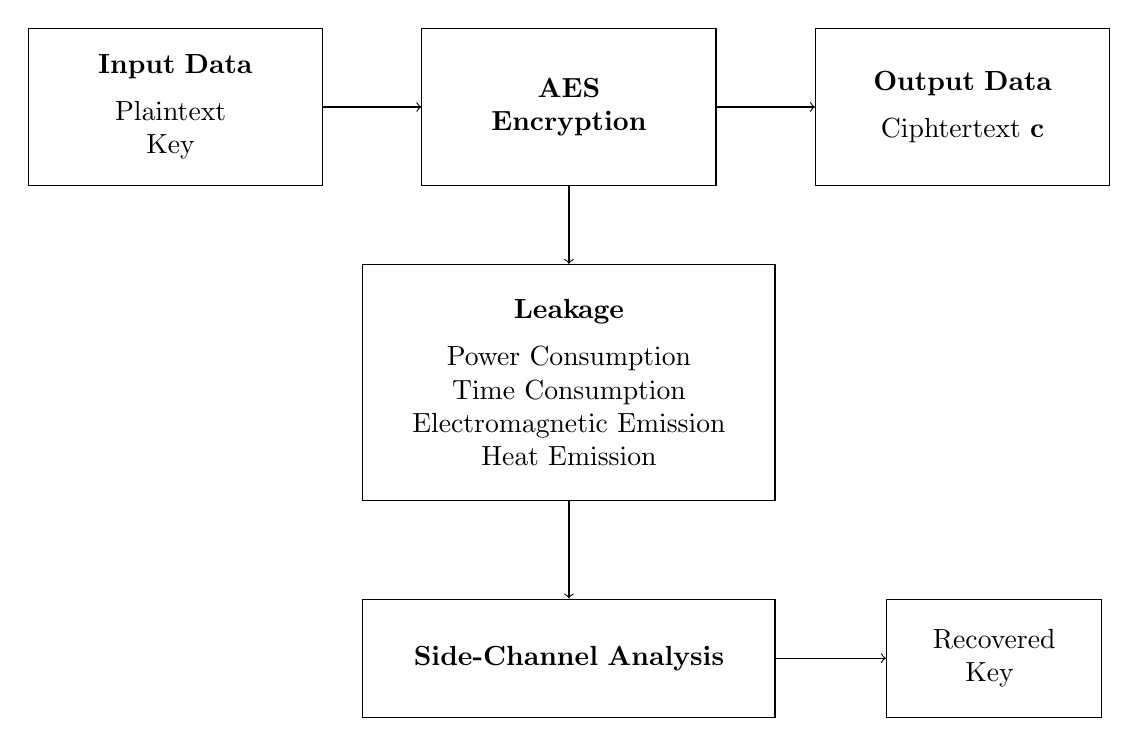
\begin{tikzpicture}%[trim left=5cm]
        \node[text width=3.5cm, align=center] (in) at (0,0) [draw,minimum width=1.5cm,minimum height=2cm] {\textbf{Input Data} \\ \vspace{0.5em} Plaintext $\pp$ \\ Key $\kk$};
        \node[text width=3.5cm, align=center] (aes) at (5,0) [draw,minimum width=1.5cm,minimum height=2cm] {\textbf{AES \\ Encryption}};
        \node[text width=3.5cm, align=center] (out) at (10,0) [draw,minimum width=1.5cm,minimum height=2cm] {\textbf{Output Data} \\ \vspace{0.5em} Ciphtertext $\mathbf{c}$};

        \node[text width=5cm, align=center] (leak) at (5,-3.5) [draw,minimum width=1.5cm,minimum height=3cm] {\textbf{Leakage} \\ \vspace{0.5em} Power Consumption \\  Time Consumption \\ Electromagnetic Emission \\ Heat Emission};
        \node[text width=5cm, align=center] (sca) at (5,-7) [draw,minimum width=1.5cm,minimum height=1.5cm] {\textbf{Side-Channel Analysis}};
        \node[text width=2.5cm, align=center] (k) at (10.4,-7) [draw,minimum width=1.0cm,minimum height=1.5cm] {Recovered \\ Key $\kk$};

        \draw[->] (in) -- (aes) node[midway,left] {};
        \draw[->] (aes) -- (out) node[midway,left] {};
        \draw[->] (aes) -- (leak) node[midway,left] {};
        \draw[->] (leak) -- (sca) node[midway,left] {};
        \draw[->] (sca) -- (k) node[midway,left] {};
\end{tikzpicture}

        }
    }%

    \caption{Schematic overview of a side-channel attack on the AES encryption function.}
    \label{fig:sca}
\end{figure}

% General
Although a cryptographic algorithm may be secure conceptually, its implementation may be not: Side-channel attacks exploit the fact that physical implementations of an algorithm unintentionally leak information about the processed data. For example, consider an encryption algorithm, that takes the plaintext and the cryptographic key as input and outputs the ciphertext. In practice, the implementation of such an algorithm also produces artifacts information that contains information about the input data, particularly the secret key \cite{scas}. For example, since the power usage of CMOS transistors depends on the switching activity during the computation, the power consumption of the device performing the encryption is not only dependent on the algorithm but also on the data processed \cite{intro_sca}. It has been frequently shown that side-channel attacks are more efficient than the best-known cryptanalytic attacks, which consider the system under attack as an idealized, mathematical model \cite{intro_sca}.
While adversaries can exploit various side channels such as timing of operations \cite{timing_kocher} and electromagnetic emanation \cite{em_gandolfi}, this work focuses on information about power consumption. A schematic overview of a side channel attack is shown in Figure \ref{fig:sca}.


% Template Attacks
\subsection{Template Attacks}
\label{sec:ta}
Consider an adversary attacking an implementation of a cryptographic algorithm running on a target device (e.g., a smart card) and assume that the attacker has access to a \textit{clone} device that is identical in hardware to the target device. If the attacker has full control over the clone device, they can arbitrarily choose the input to the algorithm (e.g., key and plaintext in a block cipher) and record the side-channel leakage of her choice (e.g., power consumption of the clone device). In this \textit{profiling} phase, they effectively build a dataset of input-leakage pairs, denoted as \textit{profiling dataset}. Since the input and the algorithm are fully known, we can reconstruct any intermediate value and the algorithm's output (assuming a deterministic algorithm).

Due to the leakages being noisy, there exists no deterministic map between processed data and leakage. A natural choice is to build a (generative) probabilistic model of this relationship: More formally, let $\leak \in \mathbb{R}^d$ denote a leakage (e.g., power trace), let $v \in \{0,\dots,255\}$ be a byte-valued variable\footnote{In this thesis, we mainly focus on distributions over \textit{bytes}. However, we discuss the applicability of our approach to other distribution scopes in Section \ref{sec:scopes}.} used in the algorithm (e.g., an input, intermediate variable, or output), and let $\dat = \{(\leak^{(i)}, v^{(i)})\}_{i=1}^n$ denote the profiling dataset. A common choice is to model the likelihood as a multivariate Gaussian, i.e.,
\begin{equation}
\label{eq:likelihood}
    p(\leak \mid v) = \mathcal{N}(\mv, \cov_v) = \frac{1}{\sqrt{(2\pi)^d \cdot |\cov_v|}} \cdot \exp\left( -\frac{1}{2} (\leak - \mv)^T \cov_v^{-1} (\leak - \mv) \right)
\end{equation}
where $\mv$ is the mean of the leakages for some value $v$, which we estimate using the \textit{Maximum Likelihood} estimator $\tilde{\mv} = \frac{1}{|\dat_v|}\sum_{\leak_v \in \dat_v}\leak_v$ where $\dat_v \subseteq \dat$ refers to the subset of the dataset where the variable of interest assumed value $v$, and $\cov_v$ is the positive semi-definite covariance matrix, estimated as 
\begin{align}
    \tilde{\cov}_v = \frac{1}{|\dat_v| - 1} \sum_{\leak_v \in \dat_v} \left( \leak_v - \tilde{\mv} \right) \left( \leak_v - \tilde{\mv} \right)^T
\end{align}

Since the leakages $\leak$ are high-dimensional in practice (e.g., $d=10^5$), one might first apply one or more dimensionality reduction techniques as pre-processing steps. For example, Bronchain et al. \cite{5min} use a combination of signal-to-noise ratio estimation to find points of interest in $\leak$ and then perform \textit{Linear Discriminant Analysis} (LDA) to linearly project the compressed leakage into a lower dimensional subspace \cite{5min}.

Consequently, the adversary constructs $256$ Gaussians (\textit{templates}) based on the profiling dataset, one for each unique value $v$.
Since the attacker is usually interested in multiple intermediate variables $v_1, \dots, v_k$, they repeat this modeling process $k$ times. 


During the attack on the target device, the attacker only has access to the leakage and wishes to infer the values of the processed data. We can turn the generative model in Equation \ref{eq:likelihood} (likelihood) into a predictive model by utilizing Bayes' law: 
\begin{equation}
\label{eq:bayes}
    p(v \mid \leak) = \frac{p(\leak \mid v) p(v)}{\sum_{v'=0}^{255} p(\leak \mid v') p(v')}
\end{equation}

Typically, the prior $p(v)$ is chosen to be uniform, which simplifies Equation \ref{eq:bayes} to

\begin{equation}
\label{eq:bayes_simple}
    p(v \mid \leak) = \frac{p(\leak \mid v)}{\sum_{v'=0}^{255} p(\leak \mid v')}
\end{equation}


We also note that while modeling distribution over \textit{byte-valued} variables $v$ is a common choice, other works investigate extending the scope of $v$ to multiple bytes (e.g., 2 bytes or 4 bytes) \cite{32bit}, or to shrink the scope of $v$ to bit-level \cite{breaking_free}.
Moreover, instead of directly predicting the \textit{value} of a particular variable $p(v \mid \leak)$, we can generalize this setup by choosing to predict a \textit{function} of the value $p(f(v) \mid \leak)$. $f(v)$ is called a \textit{leakage model} and popular choices include the \textit{Hamming weight}, i.e., the number of bits in $v$ that are set to $1$, and the identity function $f(v) = v$. 

After obtaining posterior distributions for all variables of interest $p(f(v_1) \mid \leak), \dots, p(f(v_k) \mid \leak)$, the attacker aims to aggregate their beliefs about $v_1, \dots, v_k$ to obtain distributions over the \textit{key bytes}. Intuitively, beliefs about intermediate variables depending on the key bytes should be propagated and combined into beliefs about the key itself.

% ASCA
\subsection{Algebraic Side-Channel Attacks}
\label{sec:asca}
In order to infer beliefs about the key from beliefs about intermediate values, knowledge about the cryptographic algorithm must be combined with the distributions $p(f(v_1) \mid \leak), \dots, p(f(v_k) \mid \leak)$.

One possible way to achieve this is to first transform the algorithm into a boolean representation \cite{asca}. Let $\algo$ be the cryptographic algorithm and $\mathbf{v} = (v_1, \dots, v_k)^T$ be the collection of intermediate variables used in $\algo$. Then, 
\begin{equation}
    \algo_B(\mathbf{v}) = \begin{cases}
        1 \quad \text{if $\mathbf{v}$ is consistent with $\algo$} \\
        0 \quad \text{else}
    \end{cases}
\end{equation}
is called the \textit{boolean representation} of $\algo$. 

If an attacker knew certain intermediate variables with certainty, they could represent both $\mathcal{A}_B$ and their knowledge about intermediate variables in conjunctive normal form (CNF) and use a SAT solver to deduce the key. This approach is known as an \textit{Algebraic Side-Channel Attack} (ASCA) \cite{asca}.

For example, assume that they first use a template attack to obtain $p(f(v_1) \mid \leak), \dots, p(f(v_k) \mid \leak)$ with $f(v)$ being the Hamming weight of $v$. Also assume that $p(f(v_1) = 1 \mid \leak) = 1$, i.e., they know with certainty that exactly $1$ bit of the byte $v_1$ is set to $1$. If $v_1^{(1)},\dots,v_1^{(8)}$ denote the individual bits of $v_1$, they can easily encode this leakage information into a boolean formula as follows:
\begin{equation}
    \left( v_1^{(1)} \land \bigwedge_{i \in \{2,\dots,8\}} \neg v_1^{(i)} \right) \lor \left( v_1^{(2)} \land \bigwedge_{i \in \{1,3,4,\dots,8\}} \neg v_1^{(i)} \right) \lor \dots \lor \left( v_1^{(8)} \land \bigwedge_{i \in \{1,\dots,7\}} \neg v_1^{(i)} \right)
\end{equation}
This can then be transformed into a CNF and added to the set of clauses that represent $\mathcal{A}_B$. If the adversary also knows the Hamming weight of all other intermediates with certainty, they can repeat this process and use a SAT solver to find the only valid key assignment in the final CNF.

In practice, however, we cannot extract information from the leakage about all intermediates with absolute certainty. As a remedy, the ASCA first picks the most likely Hamming weight for all intermediates and runs the attack, then proceeds to use the second most likely combination of Hamming weights, and so on \cite{asca}. If some combination of Hamming weights is inconsistent with $\mathcal{A}_B$, the resulting CNF will be unsatisfiable.

Clearly, the main downside of this attack is that the attacker has to collapse their probabilistic model about intermediate values to \textit{hard}, deterministic assumptions to be able to provide leakage information to a SAT solver. This leads to the fact that the ASCA is highly sensitive to errors - Renault et al. \cite{asca_aes} were only able to solve problems with an error rate under $1\%$, which is of limited use in practical scenarios \cite{tasca}.

% Tolerant ASCA
Consequently, attacks that are less sensitive to noise have been developed: Instead of directly using an error-intolerant SAT solver, \textit{Tolerant Algebraic Side-Channel Analysis} (TASCA) leverages Pseudo-Boolean optimization, a special case of integer programming that solves a constraint optimization problem \cite{tasca}.
The authors introduce error variables in their set of equations (which assumes a fixed upper bound on the measurement error) and instruct the solver to minimize the total number of error variables \cite{tasca}. However, this approach is still inefficient in exploiting soft information and fails if the measurement error is larger than the assumed upper bound \cite{sasca}.

\subsection{Soft Analytical Side-Channel Attacks}
\label{sec:sasca}
% Factor graph + BP
Instead of using SAT solvers or optimizers, a \textit{Soft Analytical Side-Channel Attack} (SASCA) represents a cryptographic algorithm as a \textit{factor graph}, a type of probabilistic graphical model \cite{sasca}. A factor graph is a bipartite graph, consisting of two types of nodes - namely \textit{variable nodes} and \textit{factor nodes}. A factor node represents a function and all connected variable nodes represent arguments to this function. An example is illustrated in Figure \ref{fig:example_factor_graph}.

\begin{figure}[ht]
    \begin{center}
    \scalebox{1.25}{
        \begin{tikzpicture}
    \factor[] {fa} {right:$f_a$} {} {};
    \factor[right=1 of fa] {fb} {right:$f_b$} {} {};
    \factor[right=1 of fb] {fc} {right:$f_c$} {} {};
    \factor[right=1 of fc] {fd} {right:$f_d$} {} {};
    \node[latent, above=of fa, xshift=0cm] (x1) {$x_1$} ; %
    \node[latent, right=1.07 of x1] (x2) {$x_2$} ; %
    \node[latent, right=1.07 of x2] (x3) {$x_3$} ; %
    \factoredge {x1,x2} {fa} {} ; %
    \factoredge {x1,x2} {fb} {} ; %
    \factoredge {x2,x3} {fc} {} ; %
    \factoredge {x3} {fd} {} ; %
\end{tikzpicture}

    }
    \end{center}
    \caption{A factor graph representing $f(x_1, x_2, x_3) = f_a(x_1, x_2) f_b(x_1, x_2) f_c(x_2, x_3) f_d(x_3)$.}
    \label{fig:example_factor_graph}
\end{figure}

In general, a factor graph which has factor nodes $\mathcal{F} = \{f_1,\dots,f_n\}$ and variable nodes $\mathcal{V} = \{x_1,\dots,x_m\}$ specifies a function $f(x_1,\dots,x_m) = \prod_{i=1}^n f_i(\neigh(f_i))$ where $\neigh(f)$ denotes the set of neighbours of factor $f$ (which are variable nodes). Often, factor graphs are used to represent probability mass functions or probability density functions \cite{fg_loeliger}.
The SASCA models every function used in the cryptographic implementation (e.g., \textsc{xor}, \textsc{sbox}, \textsc{xtime}) as a factor with binary output \cite{sasca}. For example,
\begin{equation}
    \textsc{xor}(a, b, c) = \begin{cases}
        1 \quad \text{if $a \oplus b = c$} \\
        0 \quad \text{else}
    \end{cases} \qquad
    \textsc{sbox}(a, b) = \begin{cases}
        1 \quad \text{if $S(a) = b$} \\
        0 \quad \text{else}
    \end{cases}
\end{equation}
where $a,b,c$ are byte-valued variables and $S$ is an \textsc{sbox} function, as found in the AES.

All variables are modeled as variable nodes and, additionally to being connected to the function nodes as described in the algorithm, each variable is connected to a factor representing the corresponding posterior distribution obtained e.g. via a template attack.
For example, consider the following excerpt of AES: 
$$y = k \oplus p, \quad x = S(y)$$
where $k$ is a key byte, $p$ is a \textit{known} plaintext byte, and $S$ as a bijection that denotes the AES S-box.
The corresponding factor graph is shown in Figure \ref{fig:xor_sbox_fg} and effectively represents an unnormalized joint probability distribution over unobserved variables, i.e.,
$$ \tilde{p}(k,y,x) = p(k | \leak) \cdot p(y | \leak) \cdot p(x | \leak) \cdot \textsc{xor}(k,p,y) \cdot \textsc{sbox}(y,x) $$
The normalized version reads
$$ p(k,y,x) = \frac{1}{Z} \ \tilde{p}(k,y,x) \quad \text{with} \quad Z = \sum_k \sum_y \sum_x \tilde{p}(k,y,x).$$ 

The goal is to obtain the \textit{marginal} of the key, i.e., compute
$$ p(k) = \sum_y \sum_x p(k,y,x).$$
A SASCA computes this quantity using \textit{Belief Propagation} (BP), an iterative message-passing algorithm that is detailed in Section \ref{sec:bp}. In a nutshell, the algorithm is guaranteed to output the exact marginal if the factor graph is a tree.
While BP can also be applied to \textit{estimate} marginals in cyclic graphs (\textit{loopy BP}), it is neither guaranteed that the algorithm converges nor that the output is an accurate estimate \cite{bp}.

\begin{figure}[ht]
    \begin{center}
    \scalebox{1.25}{
        \begin{tikzpicture}
    \factor[] {xor} {below:$\textsc{xor}$} {} {};
    \factor[right=2.5 of xor] {sbox} {below:$\textsc{sbox}$} {} {};

    \node[latent, above=of xor, xshift=-1.7cm] (k) {$k$} ; %
    \node[obs, right=1 of k] (p) {$p$} ; %
    \node[latent, right=1 of p] (y) {$y$} ; %
    \node[latent, right=1 of y] (x) {$x$} ; %
    \factoredge {k,p,y} {xor} {} ; %
    \factoredge {y,x} {sbox} {} ; %

    \factor[above=of k] {pk} {above:$p(k | \leak)$} {} {};
    \factor[above=of y] {py} {above:$p(y | \leak)$} {} {};
    \factor[above=of x] {px} {above:$p(x | \leak)$} {} {};

    \factoredge {k} {pk} {} ; %
    \factoredge {y} {py} {} ; %
    \factoredge {x} {px} {} ; %

\end{tikzpicture}

    }
    \end{center}
    \caption{A factor graph that incorporates both the posterior distributions over unobserved variables, as well as the algorithmic relationship between variables. Note that the plaintext $p$ is assumed to be known.}
    \label{fig:xor_sbox_fg}
\end{figure}

\subsection{Belief Propagation}
\label{sec:bp}

The following exposition closely follows the work of Christopher Bishop \cite{bishop}.
Assume we are given a factor graph that is connected (i.e., there exists a path between any two nodes), and contains no cycles (i.e., there exists no sequence of distinct edges that form a path that starts and ends at the same). This factor graph contains a collection of variables $\xx$ and we wish to compute the marginal 
\begin{equation}
    p(x) = \sum_{\xx \setminus x} p(\xx)
\end{equation}
for a particluar $x$, where $\xx \setminus x$ denotes all variables in $\xx$, except $x$.

\begin{figure}[ht]
    \centering
    \scalebox{1.25}{
        \begin{tikzpicture}
    \node[xshift=-1.2cm, yshift=0.2cm, cloud, draw, fill = gray!10, minimum width = 4.5cm, minimum height = 4.5cm] {};
    \factor[] {fs} {below:$f_s$} {} {}; %
    \node[latent, left=of fs, yshift=0.7cm] (x1) {} ; %
    \node[latent, below=1cm of x1] (x2) {} ; %
    \node[above=0.2cm of x2] {$\vdots$};

    \node[latent, right=3.3cm of fs] (x) {$x$} ; %
    \factor[right=1cm of x, yshift=0.7cm] {f1} {} {} {}; %
    \factor[below=1cm of f1] {f2} {} {} {}; %
    \node[above=0.2cm of f2] {$\vdots$};

    \node[above=0.05cm of fs, xshift=2.1cm] {$\underrightarrow{\rule[-6pt]{0pt}{2pt}{\mu_{f_s \to x}(x)}}$};
    \node[above=0.05cm of x1, xshift=0.3cm, yshift=0.12cm] {$F_s(x, \xx_s)$};


    \factoredge {x1,x2} {fs} {} ; %
    \factoredge {x} {f1,f2,fs} {} ; %
\end{tikzpicture}

    }
    \caption{Subtree $F_s$ connected to variable node $x$.}
    \label{fig:fac_to_var}
\end{figure}

As illustrated in Figure \ref{fig:fac_to_var}, the variable node $x$ is connected to one or more factor nodes, each of which can be viewed as the root of a particular subtree. Let $f_s$ be any neighbour\footnote{$f_s$ is guaranteed to be a factor node since the factor graph is bipartite.} of $x$ and let $F_s(x, \xx_s)$ be the subtree connected to $f_s$, where $\xx_s$ is the subset of variables in $\xx$ that can be found in subtree $F_s$. With $\neigh(x)$ denoting the set of factor nodes that are neighbours of $x$, we can write 
\begin{equation}
    p(\xx) = \prod_{s \in \neigh(x)} F_s(x, \xx_s)
\end{equation}
 which simply expresses the factorization as a product of subtrees (which are themselves products). Thus,
\begin{align}
    p(x) = \sum_{\xx \setminus x} p(\xx) &= \sum_{\xx \setminus x} \ \prod_{s \in \neigh(x)} F_s(x, \xx_s) \\
         &= \prod_{s \in \neigh(x)} \underbrace{\sum_{\xx_s} F_s(x, \xx_s)}_{\mu_{f_s \to x}(x)}
\end{align}

where we define $\mu_{f_s \to x}(x) = \sum_{\xx_s} F_s(x, \xx_s)$ to be a \textit{message} from $f_s$ to $x$.
Note that we are only allowed to pull the sum into the product since for any two $s, s' \in \neigh(x)$, the sets $\xx_s$ and $\xx_{s'}$ are disjoint (since the factor graph is a tree).

\begin{figure}[ht]
    \centering
    \scalebox{1.25}{
        \begin{tikzpicture}
    \node[xshift=-3.2cm, yshift=1.2cm, cloud, draw, fill = gray!10, minimum width = 2.5cm, minimum height = 2.5cm] {};
    \factor[] {fs} {below:$f_s$} {} {}; %
    \node[latent, left=3cm of fs, yshift=0.7cm] (x1) {$x_i$} ; %
    \node[latent, below=1cm of x1] (x2) {$x_m$} ; %
    \node[above=0.02cm of x2] {$\vdots$};

    \node[latent, right=2cm of fs] (x) {$x$} ; %
    \factor[right=1cm of x, yshift=0.7cm] {f1} {} {} {}; %
    \factor[below=1cm of f1] {f2} {} {} {}; %
    \node[above=0.2cm of f2] {$\vdots$};

    \node[above=0.05cm of fs, xshift=1.1cm] {$\underrightarrow{\rule[-6pt]{0pt}{2pt}{\mu_{f_s \to x}(x)}}$};
    \node[above=0.05cm of x1, xshift=0.3cm, yshift=0.01cm] {$G_s(x_i, \xx_{si})$};

    \node[right=0.15cm of x2, yshift=-0.4cm, label={[rotate=17]right:$\overrightarrow{\rule[6pt]{0pt}{4pt}{\mu_{x_m \to f_s}(x_m)}}$}] {}; 

    \factoredge {x1,x2} {fs} {} ; %
    \factoredge {x} {f1,f2,fs} {} ; %
\end{tikzpicture}

    }
    \caption{Within $F_s$, we have subtrees $G_s$ connected to factor node $f_s$.}
    \label{fig:var_to_fac}
\end{figure}

As shown in Figure \ref{fig:var_to_fac}, $F_s(x, \xx_s)$ can be decomposed similarly by looking at all subtrees in $F_s$ that are connected to $f_s$:
\begin{align}
    F_s(x, \xx_s) = f_s(x, x_1, \dots, x_m) G_1(x_1, \xx_{s1}) \cdots G_m(x_m, \xx_{sm})
\end{align}
where $\xx_{si}$ denotes the set of variables in subtree $G_i$, apart from $x_i$, the direct neighbour of $f_s$.
Hence,
\begin{align}
\label{eq:bp_ftv}
    \mu_{f_s \to x}(x) &= \sum_{\xx_s} \left( f_s(x, x_1,\dots,x_m) \prod_{i \in \neigh(f_s) \setminus x} G_i(x_i, \xx_{si}) \right) \\
    &= \sum_{x_1,\dots,x_m} f_s(x, x_1,\dots,x_m) \prod_{i \in \neigh(f_s) \setminus x} \underbrace{\left( \sum_{\xx_{si}} G_i(x_i, \xx_{si}) \right)}_{\mu_{x_i \to f_s}(x_i)}
\end{align}
where $\mu_{x_i \to f_s}(x_i)$ can be viewed as a message from variable node $x_i$ to factor node $f_s$.

\begin{figure}[ht]
    \centering
    \scalebox{1.25}{
        \begin{tikzpicture}
    \node[xshift=-2.6cm, yshift=1.3cm, cloud, draw, fill = gray!10, minimum width = 2.3cm, minimum height = 2.3cm] {};
    \factor[] {fs} {below:$f_s$} {} {}; %
    \node[latent, left=1cm of fs] (x) {$x_i$} ; %
    \factor[left=1cm of x, yshift=0.7cm] {fl} {$f_l$} {} {}; %
    \factor[below=1.5cm of fl] {fL} {$f_L$} {} {}; %
    \node[above=0.5cm of fL] {$\vdots$}; %

    \node[above=0.45cm of fl, xshift=0.3cm, yshift=0.01cm] {$F_l(x_i, \xx_{il})$};
    \factoredge {x} {fl,fL,fs} {} ; %
\end{tikzpicture}

    }
    \caption{Within $G_s$, we again have subtrees $F_l$ connected to variable node $x_i$.}
    \label{fig:gi}
\end{figure}

As Figure \ref{fig:gi} shows, we can again decompose the graph $G_i(x_i, \xx_{si})$ into subgraphs in $G_i$ that are connected to $x_i$:
\begin{align}
    G_i(x_i, \xx_{si}) = \prod_{l \in \neigh(x_i) \setminus f_s} F_l(x_i, \xx_{il})
\end{align}
and therefore, the variable-to-factor message can be computed as
\begin{align}
    \mu_{x_i \to f_s}(x_i) = \sum_{\xx_{si}} G_i(x_i, \xx_{si}) &= \sum_{\xx_{si}} \left( \prod_{l \in \neigh(x_i) \setminus f_s} F_l(x_i, \xx_{il}) \right) \\ 
    &= \prod_{l \in \neigh(x_i) \setminus f_s} \underbrace{\left( \sum_{\xx_{il}} F_l(x_i, \xx_{il}) \right)}_{\mu_{f_l \to x_i}(x_i)}
\end{align}
%which completes the recursion.

In short, to compute variable-to-factor messages, we take the product of all incoming factor-to-variable messages. To compute factor-to-variable messages, we sum over the product of the factor and the incoming variable-to-factor messages.
If the node is a leaf (i.e., it has a single connection to another node), we set $\mu_{x \to f}(x) = 1$ if the leaf is a variable node and $\mu_{f \to x}(x) = f(x)$ if the leaf is a factor node.

In order to compute the marginal $p(x)$, we start by viewing the variable node $x$ as the root of the tree. Starting from the leaves, we recursively send messages along the (unique) path towards the root node. As soon as the root node has received all messages from its neighbours, we multiply the messages and re-normalize them to obtain $p(x)$ \cite{bishop}. If we are interested in all other marginals, we can compute them in a subsequent single downward pass (i.e., from the root towards the leaves) \cite{bishop}.

As long as the factor graph is a tree, BP computes the exact marginals \cite{bp}. In general, as soon as we introduce cycles in the graph, BP has (1) no guarantee of convergence, and even if it converges, (2) has no guarantee of computing an accurate estimate of the true marginals \cite{bp}.

%To complete the recursion

\section{Probabilistic Circuits}
% Why probabilistic modeling?
Probabilistic models are central objects in machine learning (ML) and artificial intelligence (AI). Probability theory provides a principled, sound and consistent way to reason under uncertainty. If we knew the \textit{true} data-generating probability distribution, many tasks in ML reduce to \textit{probabilistic inference} \cite{pc_intro}.

% General, class of tractable models
Probabilistic Circuits (PCs) represent a class of probabilistic models. In essence, they can be viewed as parameterized functions that represent probability distributions (discrete, continuous, or a mix of both). However, when compared to other probabilistic models such as (deep) generative models and probabilistic graphical models, PCs leverage certain structural properties in order to answer classes of inference queries (such as marginals, conditionals or maximizations) exactly and efficiently, i.e., in time polynomial in the size of the circuit \cite{pc_intro}. 
In general, the more structure we impose on a circuit, the more classes of queries we can hope to answer \emph{tractably} (i.e., efficiently) \cite{compositional_atlas}.

PCs can be considered as computational graphs that recursively mix (\textit{sum nodes}) and factorize (\textit{product nodes}) simpler parametric distributions (e.g., Bernoullis or Gaussians) that are located at the leaves of the graph. An example PC is shown in Figure \ref{fig:example_pc}.

% leaves: simple prob distributions
% non-leaves: 

\begin{figure*}[ht!]
    \begin{subfigure}[t]{0.6\textwidth}
        \centering
        \begin{tikzpicture}

    \node[latent] (ptop) {$+$} ; %
    \node[latent, below=0.8cm of ptop, xshift=-1.3cm] (xleft) {$\times$} ; %
    \node[latent, right=2cm of xleft] (xright) {$\times$} ; %
    \edge[-] {xleft, xright} {ptop}

    \node[above=0.2cm of xleft, xshift=0.4cm] {$w_1$};
    \node[above=0.2cm of xright, xshift=-0.5cm] {$w_2$};

    % leafs
    \node[latent, below=0.8cm of xleft, xshift=-0.7cm] (a1_left) {$A$} ; %
    \node[latent, right=0.7cm of a1_left] (b1_left) {$B_\theta$} ; %
    \edge[-] {a1_left, b1_left} {xleft} ; %

    \node[latent, below=0.8cm of xright, xshift=-0.7cm] (a1_right) {$\neg A$} ; %
    \node[latent, right=0.7cm of a1_right] (b1_right) {$B$} ; %
    \edge[-] {a1_right, b1_right} {xright} ; %

\end{tikzpicture}

    \end{subfigure}
    ~
    \begin{subfigure}[t]{0.4\textwidth}
        \vspace{-3.2cm}
        % \centering
        \begin{tabular}{cc|l}
           $A$ & $B$ & $p(A, B)$ \\
           \hline
           $0$ & $0$ & $0$ \\
           $0$ & $1$ & $w_2$ \\
           $1$ & $0$ & $w_1 (1 - \theta)$ \\
           $1$ & $1$ & $w_1 \theta$
        \end{tabular}
    \end{subfigure}
    \caption{A PC over 2 binary random variables $A, B$ with parameters $\{w_1, w_2, \theta\}$. Let $\mathcal{B}(\pi)$ denote a Bernoulli distribution with success probability $\pi$. For the 4 leaf distributions, we use a shorthand notation and write $A$ to mean $p_1(A) = \mathcal{B}(1)$, $B_\theta$ to mean $p_2(B) = \mathcal{B}(\theta)$, $\neg A$ to mean $p_3(A) = \mathcal{B}(0)$, and $B$ to mean $p_4(B) = \mathcal{B}(1)$.}
    \label{fig:example_pc}
\end{figure*}

% Smoothness, (structured) decomposability, determinism
\begin{definition}[Scope]
If a PC defines a joint distribution over a set of variables $\xx$, each node can be seen as the root of a subgraph that models a distribution over a subset of $\xx$. This subset is called the \textit{scope} of the node, denoted $\phi(n)$ where $n$ is a node in the PC. The scope of a leaf node is the set of input variables the base distribution models. If a node is not a leaf, its scope is given by the union of its children's scopes: $\phi(n) = \cup_j \phi(\inp(n)_j)$ with $\inp(n)$ denoting the vector of input nodes that feed into $n$. Hence, the root node $r$ always has scope $\phi(r) = \xx$. 
\end{definition}

\begin{definition}[Size]
    The \textit{size} of a PC is the number of edges in the corresponding computational graph.
\end{definition}
\begin{definition}[Smoothness]
    A sum node is \textit{smooth} if all its inputs have the same scope. A PC is smooth if all its sum nodes are smooth.
\end{definition}
\begin{definition}[Decomposability]
    A product node is \textit{decomposable} if all its inputs have disjoint scopes, i.e., they do not share variables. A PC is decomposable if all of its product nodes are decomposable.
\end{definition}
\begin{definition}[Determinism]
    A sum node is \textit{deterministic} if, for any fully-instantiated input, at most one of its children assumes a non-zero value. A PC is deterministic if all sum nodes are deterministic.
\end{definition}

The PC shown in Figure \ref{fig:example_pc} is smooth, decomposable and deterministic. 

Consider the PC shown in Figure \ref{fig:example_pc}. To compute $p(A,B)$ for a particular assignment, say $A=0, B=1$, we evaluate the circuit bottom-up: First, we evaluate the probability mass functions at the leaves, yielding $p_1(A=0) = 0, p_2(B=1)=\theta, p_3(A=0)=1, p_4(B=1)=1$ (from left to right). Then, we perform the multiplications $0 \cdot \theta$ and $1 \cdot 1$ and feed the output in the weighted sum node at the root, computing $w_1 \cdot 0 + w_2 \cdot 1 = w_2 = p(A=0, B=1)$.

\begin{theorem}[Tractable Marginal Queries]
\label{theorem:tractable_marginal}
    A smooth and decomposable PC representing a joint distribution $p(\xx)$ can compute any marginal distribution $p(\xx_s) = \sum_{\xx \setminus \xx_s} p(\xx)$ in linear time in the size of the circuit.\footnote{In this work, we are only concerned with discrete probability distributions. However, in general, smooth and decomposable PCs can also compute marginals over continuous densities, i.e., integrals.}
\end{theorem}
We show a proof for this theorem in Appendix \ref{app:tractable_marginal_proof}.

\begin{theorem}[Tractable MPE Queries]
\label{theorem:tractable_mpe}
    A smooth, decomposable and \textit{deterministic} PC representing a joint distribution $p(\xx)$ can compute \textit{most probable evidence} (MPE) queries $\argmax_{\xx} p(\xx)$ in linear time in the size of the circuit.
\end{theorem}
We prove this theorem in Appendix \ref{app:tractable_mpe_proof}.

% structured decomp & vtree
\begin{definition}[Structured Decomposability]
    Given a PC whose product nodes all have exactly two inputs,\footnote{Every PC can be converted into a circuit that fulfills this condition in exchange for a polynomial increase in size \cite{compositional_atlas}.} we call this PC \textit{structured decomposable} if it is decomposable and every pair of product nodes $n_1, n_2$ with the same scope decompose in the same way: $(\phi(n_1) = \phi(n_2)) \Rightarrow (\forall j: \phi(\inp(n_1)_j) = \phi(\inp(n_2)_j))$ \cite{pc_intro}.
\end{definition}

Of course, there are many decompositions to choose from (each of which gives a different PC). We will now introduce an object that specifies a particular decomposition for every product node, a so-called \textit{vtree}.

\begin{definition}[Vtree]
    A \textit{vtree}, or \textit{variable tree}, is a full, rooted binary tree whose leaves are in a one-to-one correspondence to the variables in the PC \cite{new_comp_lang}.
\end{definition}

\begin{figure}[ht]
    \centering
    \scalebox{1.25}{
        \begin{tikzpicture}
    \node[] (dot) {$\cdot$} ; %
    \node[below=0.5cm of dot, xshift=-0.55cm] (a) {$A$} ; %
    \node[right=0.5cm of a] (b) {$B$} ; %
    \edge[-] {a, b} {dot}; %
\end{tikzpicture}
    }
    \caption{The unique vtree corresponding to the structured decomposable PC in Figure \ref{fig:example_pc}.}
    \label{fig:vtree_example}
\end{figure}

Figure \ref{fig:vtree_example} shows the vtree that corresponds to the PC shown in Figure \ref{fig:example_pc} (we say that the PC \textit{respects} this vtree). For every product node in the PC, the decomposition of its scope is governed by exactly one \textit{internal} node in the vtree. In this example, there is only one internal vtree node.
% PSDD

\section{Knowledge Compilation}

We can represent knowledge bases (i.e., statements in propositional logic) using different \emph{languages}, which impose different structural constraints on the representation of statements \cite{kcm}. For example, \emph{Conjunctive Normal Form} (CNF) and \emph{Disjunctive Normal Form} (DNF) are two well-known languages \cite{kcm}. Importantly, a language must trade-off (1) how compactly it can represent a given knowledge base and (2) the class of \emph{queries} it supports in polytime \cite{kcm}. For example, consider a knowledge base that is represented in both CNF and DNF. If we wish to enumerate all satisfying assignments (models), we observe that the DNF representation admits an answer to this query in polytime, while the CNF representation does not. The process of converting a knowledge base from one language (representation) to another is called \emph{Knowledge Compilation}.

Again consider the PC in Figure \ref{fig:example_pc}: \textit{By construction} of the circuit, the assignment $A=0, B=0$ will always have zero probability --- no matter what parameters $w_1, w_2, \theta$ we choose.
We will now describe a principled way to build PCs that define distributions over the \textit{models of a given propositional theory}.

% SDD (extends OBDD)
\subsection{Sentential Decision Diagrams}
Consider a boolean formula $f(\zz)$ that maps instantiations of a set of binary variables $\zz$ to either $\bot$ or $\top$. Given an instantiation $\zz$, we can compute if $f$ is satisfied (i.e., f outputs $\top$) by iteratively deciding on single variables $z \in \zz$: For example, consider $f(A,B) = A \lor B$. To evaluate $f$ for a given assignment for $A,B$, we may first check if $A = \top$: If so, we can immediately return $\top$. Otherwise, we must check if $B = \top$. If so, we return $\top$, otherwise $\bot$. This decision process can be represented by a \emph{binary decision tree}, which can easily be turned into an \emph{Ordered Binary Decision Diagram} (OBDD) by eliminating redundancies in the decision tree \cite{obdd}.
A \emph{Sentential Decision Diagram} (SDD) extends the notion of an OBDD: While in OBDDs, decisions are based on \emph{single variables}, SDDs can decide on entire \textit{sentences}, making them a strict superset of OBDDs \cite{sdd}. An SDD that represents the example above is shown in Figure \ref{fig:sdd_example}. Moreover, it has been shown that SDDs are exponentially more succinct than OBDDs, i.e., there exists a family of boolean functions where each member has polynomial SDD size, but exponential OBDD size \cite{sdd_vs_obdd}. An SDD can be seen as a type of logical circuit and, as we will later see, is closely related to PCs.

% partitions
\begin{definition}[Compressed Partitions]
Let $f(\xx, \yy)$ be a boolean function over disjoint sets of variables $\xx$ and $\yy$. For any such $f$, we can write $f = (p_1(\xx) \land s_1(\yy)) \lor \dots \lor (p_k(\xx) \land s_k(\yy))$ and we call $p_i$ \textit{primes} and $s_i$ \textit{subs} \cite{sdd, psdd}. Moreover, we can construct this decomposition in a way that $p_i \land p_j = \bot$ for $i \neq j$, $p_1 \lor \dots \lor p_k = \top$, and $p_i \neq \bot$ for all $i$. Further, we restrict the subs to be distinct, i.e., $s_i \neq s_j$ for all $i \neq j$. We call $\{(p_1,s_1),\dots,(p_k,s_k)\}$ a \textit{compressed $\xx$-partition} of $f$ \cite{sdd}.
\end{definition}

\begin{figure*}[h!]
    \begin{subfigure}[t]{0.6\textwidth}
        \centering
        \begin{tikzpicture}

    \node[latent] (ptop) {$\lor$} ; %
    \node[latent, below=0.8cm of ptop, xshift=-1.3cm] (xleft) {$\land$} ; %
    \node[latent, right=2cm of xleft] (xright) {$\land$} ; %
    \edge[-] {xleft, xright} {ptop}

    % leafs
    \node[latent, below=0.8cm of xleft, xshift=-0.7cm] (a1_left) {$A$} ; %
    \node[latent, right=0.7cm of a1_left] (b1_left) {$\top$} ; %
    \edge[-] {a1_left, b1_left} {xleft} ; %

    \node[latent, below=0.8cm of xright, xshift=-0.7cm] (a1_right) {$\neg A$} ; %
    \node[latent, right=0.7cm of a1_right] (b1_right) {$B$} ; %
    \edge[-] {a1_right, b1_right} {xright} ; %

\end{tikzpicture}

    \end{subfigure}
    ~
    \begin{subfigure}[t]{0.4\textwidth}
        \vspace{-3.2cm}
        % \centering
        \begin{tabular}{cc|l}
           $A$ & $B$ & $f(A, B)$ \\
           \hline
           $0$ & $0$ & $0$ \\
           $0$ & $1$ & $1$ \\
           $1$ & $0$ & $1$ \\
           $1$ & $1$ & $1$
        \end{tabular}
    \end{subfigure}
    \caption{An SDD representing $f(A, B) = (A \land \top) \lor (\neg A \land B) = A \lor B$. Note that we cannot directly attach $A$ and $B$ to an \textit{or} node since this would violate the smoothness property of the circuit.}
    \label{fig:sdd_example}
\end{figure*}

\begin{definition}[SDD]
    Let $v$ be a vtree over binary variables $\zz$.
    A \emph{Sentential Decision Diagram} (SDD) is a computational graph where each internal node is either a $\lor$-node (\emph{logical or}) or a $\land$-node (\emph{logical and}), while leaf nodes correspond to variables, their negation, $\top$ (true), or $\bot$ (false) \cite{sdd}. W.l.o.g., we demand that every $\lor$-node $n$ has $k \geq 1$ $\land$-nodes as children, denoted $n_1,\dots,n_k$. Each $n_i$ has exactly two children, denoted $p_i$, $s_i$. Then, $n$ represents a boolean function $g_n(\xx, \yy)$ (where $\xx, \yy$ are disjoint sets of binary variables) such that $\{(p_i,s_i)\}_{i=1}^k$ is a compressed $\xx$-partition of $g_n$. Further, there exists a node $v'$ in the vtree $v$ such that $\xx = v'_l, \yy = v'_r$ where $v'_l, v'_r$ denote the set of variables mentioned in the left and right subtree of $v'$, respectively. We say that $n$ is \emph{normalized} w.r.t. $v'$.
    Moreover, we say that an SDD \emph{respects} a vtree $v$ iff every $\lor$-node $n$ in the SDD is \emph{normalized} w.r.t. a vtree node in $v$.
\end{definition}

For example, the SDD $\lor$-node in Figure \ref{fig:sdd_example} has two primes $A, \neg A$, and two subs $B_\theta, B$. In essence, primes form a partition of the space of assignments and lead to deterministic circuits.


% sdd are canoncial -> vtree search
For a given boolean function $f$ and vtree, we can construct an SDD that is \textit{unique} (canonical SDD). Since the size of the resulting SDD heavily depends on the vtree, minimizing the size of the SDD amounts to finding a good vtree for $f$ \cite{sdd, dynamic_min_choi}. If $f$ is in \textit{Conjunctive Normal Form} (CNF), has $n$ variables and treewidth $w$, there exists a canonical SDD of size $O(n 2^w)$ \cite{sdd}.

% Compiling a CNF into an SDD is discussed in more detail in Section \ref{sec:cnf}

Since SDDs can be combined using any boolean operation in polytime \cite{sdd}, we can compile a CNF $f$ into an SDD by first constructing a circuit for each clause (which is trivial), followed by conjoining the resulting SDDs \cite{sdd}.

% PSDD
\subsection{Probabilistic Sentential Decision Diagrams}

It helps to think of SDDs as a kind of \textit{unnormalized} PC, which we can easily turn into a proper PC by (1) replacing all \textit{and} nodes with product nodes, (2) replacing all \textit{or} nodes with sum nodes (with convex weights), and (3) replacing $\top$ leaf nodes with Bernoulli distributions with a free parameter $\theta$ \cite{psdd}.
The resulting circuit is a special case of a PC that is smooth, structured decomposable, and deterministic and was introduced under the name \textit{Probabilistic Sentential Decision Diagram} (PSDD) \cite{psdd}.
For example, the SDD shown in Figure \ref{fig:sdd_example} was turned into the PSDD shown in Figure \ref{fig:example_pc}.

Clearly, no matter how we parameterize a PSDD, it can only assign a positive probability mass to variable assignments that satisfy the original formula $f$ we compiled into the underlying SDD.

It follows from the definition of an SDD that every sum node in a PSDD has one or multiple product nodes as children, all of which have exactly two inputs, which are again termed \textit{primes} (left children) and \textit{subs} (right children).

% Knowledge <=> symbolic contraints
% CNF
% SDD compiler (CNF -> SDD)

\section{Circuit Multiplication}
\label{sec:trac_op}
% Circuit Multiplication
Consider a set of variables $\xx$ and two PSDDs (i.e., smooth, structured decomposable, and deterministic PCs) $p(\yy)$ and $q(\zz)$ with $\yy, \zz \subseteq \xx$ and sizes $|p|, |q|$, respectively. We wish to also represent the \textit{product} $f(\xx) = p(\yy) \cdot q(\zz)$ as a PSDD (\textit{circuit multiplication}). In this work, we will consider probability distributions that can be written as a product of factors. As we will later see, we can first (1) compile the individual factors into PCs and (2) use circuit multiplication to multiply the factors on the circuit level. We will then use the resulting PSDD to perform inference operations.

\begin{definition}[Vtree Projection]
    Let $v$ bet a vtree over variables $\xx$. To project $v$ onto variables $\yy \subseteq \xx$, we successively remove every maximal subtree $v_0$ whose variables are not in $\yy$, while replacing the parent of $v_0$ with its sibling \cite{sbn}.
\end{definition}

% Projected vtree
\begin{figure*}[ht!]
    \begin{subfigure}[t]{0.6\textwidth}
        \centering
        \begin{tikzpicture}
    \node[] (dot) {$\cdot$} ; %
    \node[below=0.5cm of dot, xshift=-0.95cm] (a) {$\cdot$} ; %
    \node[right=1.7cm of a] (b) {$\cdot$} ; %

    \node[below=0.5cm of a, xshift=-0.55cm] (al) {$A$} ; %
    \node[right=0.5cm of al] (bl) {$B$} ; %
    \edge[-] {a, b} {dot}; %
    \edge[-] {al, bl} {a}; %
    
    \node[below=0.5cm of b, xshift=-0.55cm] (c) {$C$} ; %
    \node[right=0.5cm of c] (ddot) {$\cdot$} ; %
    \edge[-] {c, ddot} {b}; %
    
    \node[below=0.5cm of ddot, xshift=-0.55cm] (d) {$D$} ; %
    \node[right=0.5cm of d] (e) {$E$} ; %
    \edge[-] {d, e} {ddot}; %
\end{tikzpicture}

    \end{subfigure}
    ~
    \begin{subfigure}[t]{0.4\textwidth}
        \vspace{-3.2cm}
        % \centering
        \begin{tikzpicture}
    \node[] (dot) {$\cdot$} ; %
    \node[below=0.5cm of dot, xshift=-0.45cm] (a) {$A$} ; %
    \node[right=0.5cm of a] (b) {$\cdot$} ; %

    \edge[-] {a, b} {dot}; %
    
    \node[below=0.5cm of b, xshift=-0.55cm] (c) {$C$} ; %
    \node[right=0.5cm of c] (ddot) {$D$} ; %
    \edge[-] {c, ddot} {b}; %
\end{tikzpicture}
    \end{subfigure}
    \caption{A vtree (left) and its projection onto $\{A,C,D\}$ (right).}
    \label{fig:vtree_projection}
\end{figure*}

Crucially, multiplying PSDDs is tractable: If $p$ respects vtree $v_p$ and $q$ respects vtree $v_q$, $f$ can be computed in $O(|p| \cdot |q|)$ if $v_p$ and $v_q$ are projections of a common vtree $v$ and $|p|, |q|$ denote the size of $p$ and $q$, respectively \cite{tractable_ops}. We say that $p$ and $q$ are \textit{compatible}. In general, $f(\xx)$ is not a distribution but must be divided by its normalization constant $\kappa = \sum_{\xx} f(\xx)$, which can easily be computed during circuit multiplication without altering the asymptotic time complexity \cite{tractable_ops}.
While multiplying two circuits takes quadratic time, we note that in general, multiplying $N$ PSDDs is therefore exponential in $N$.

% TODO: circuit multiplication? 
Appendix \ref{app:circuit_mult} describes an algorithm that performs circuit multiplication of two PSDDs in quadratic time. While this algorithm assumes that both PSDDs are normalized w.r.t. the same vtree, this can be extended to projections of a common vtree without changing the asymptotic time complexity \cite{tractable_ops}.

\section{Entropy and Kullback-Leibler Divergence}
In this work, we will analyze approximations of probability mass functions by means of information-theoretic measures, such as \textit{Entropy} and \textit{Kullback-Leibler Divergence}.

\begin{definition}[Entropy]
    Let $p(\xx)$ be a probability mass function over variables $\xx$. The entropy $H(p)$ is defined as 
    \begin{align}
        H(p) = \expect \left[ -\log \left( p(\xx) \right) \right] = -\sum_{\xx} p(\xx) \cdot \log \left( p(\xx) \right)
    \end{align}
\end{definition}
Informally, this quantifies the \textit{expected information} about $\xx$, according to $p$.
If $p$ is a uniform distribution, i.e., $\forall \xx \in \mathcal{X}: p(\xx) = \frac{1}{|\mathcal{X}|}$, then $H(p)$ is maximized. On the other hand, if all probability mass is concentrated on a single point, i.e., $\exists \xx \in \mathcal{X}: p(\xx) = 1$, then $H(p) = 0$. Accordingly, we can interpret $H$ as a measure of diffusion.

\begin{definition}[Kullback-Leiber Divergence]
    Let $p(\xx), q(\xx)$ be probability mass functions over variables $\xx$. The \textit{Kullback-Leibler (KL) Divergence} between $p$ and $q$, written\footnote{We sometimes abuse notation and write $D_{KL}(p(\xx) \ || \ q(\xx))$ to emphasize the set of variables the distributions depend on, respectively.} $D_{KL}(p || q)$, is defined as 
    \begin{align}
        D_{KL}(p || q) = \expect_p \left[ \log \left( \frac{p(\xx)}{q(\xx)} \right) \right] = \sum_{\xx} p(\xx) \cdot \log \left( \frac{p(\xx)}{q(\xx)} \right)
    \end{align}
    where we demand that $\forall \xx: (p(\xx) > 0) \Rightarrow (q(\xx) > 0)$, i.e., the support of $q$ must not be smaller than the support of $p$.
\end{definition}
Note that $D_{KL}(p || q)$ is non-negative for any $p,q$ and is only $0$ if and only if $p,q$ are identical, i.e., $\forall \xx: p(\xx) = q(\xx)$.